\fancyhead[L]{\small\textsf{\textbf{\color{stewartcyan}MỤC 1.2}}\hspace{1em}\textsf{Mô hình Toán học: Danh mục các Hàm số Cơ bản}}
\fancyhead[R]{\small\textsf{\textbf{27}}}

\noindent
\begin{minipage}[t]{0.26\textwidth}
    \vspace{10.0cm}
    \noindent
    \small
    Một \textbf{họ hàm số} là một tập hợp các hàm số mà phương trình của chúng có mối liên hệ với nhau. Hình 12 thể hiện hai họ hàm lũy thừa, một họ với số mũ chẵn và một họ với số mũ lẻ.

    \vspace{1.8cm}
    \noindent
    \textbf{\textsf{HÌNH 12}}
\end{minipage}%
\hfill
\begin{minipage}[t]{0.71\textwidth}
    \noindent
    Công thức nghiệm của phương trình bậc hai cho ta
    \[
    t = \frac{-0.96 \pm \sqrt{(0.96)^2 - 4(-4.90)(449.36)}}{2(-4.90)}
    \]
    Nghiệm dương là $t \approx 9.67$, vì vậy chúng ta dự đoán rằng quả bóng sẽ chạm đất sau khi rơi khoảng $9.7$ giây. \hfill {\color{stewartcyan}$\blacksquare$}

    \vspace{0.33cm}
    \noindent
    {\color{stewartcyan}\rule{1.2ex}{1.2ex}}\hspace{0.5em}\textbf{\textsf{\Large Hàm lũy thừa}}

    \vspace{0.16cm}
    \noindent
    Một hàm số có dạng $f(x) = x^a$, trong đó $a$ là một hằng số, được gọi là một \textbf{hàm lũy thừa} (\textit{power function}). Chúng ta xét một vài trường hợp sau.

    \vspace{0.2cm}
    \noindent
    \textbf{\textsf{(i)}} $\boldsymbol{a = n}$, \textbf{trong đó} $\boldsymbol{n}$ \textbf{là một số nguyên dương}

    \vspace{0.12cm}
    \noindent
    Đồ thị của các hàm số $f(x) = x^n$ với $n = 1, 2, 3, 4$ và $5$ được biểu diễn trong Hình 11. (Đây là các đa thức chỉ có duy nhất một số hạng.) Chúng ta đã biết dạng đồ thị của $y = x$ (đường thẳng đi qua gốc tọa độ có hệ số góc bằng 1) và $y = x^2$ [parabol, xem Ví dụ 1.1.2(b)].

    \vspace{0.25cm}
    \noindent
    \begin{center}
        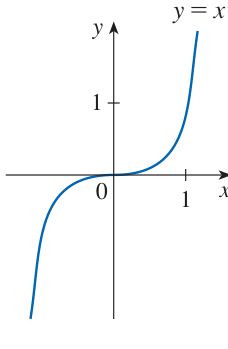
\includegraphics[width=0.185\linewidth]{images/p0062_fig1.png}\hfill
        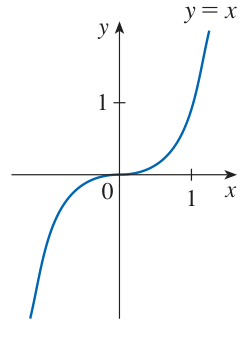
\includegraphics[width=0.185\linewidth]{images/p0062_fig2.png}\hfill
        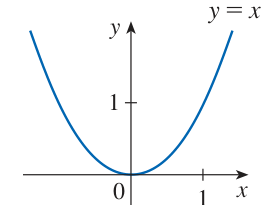
\includegraphics[width=0.185\linewidth]{images/p0062_fig3.png}\hfill
        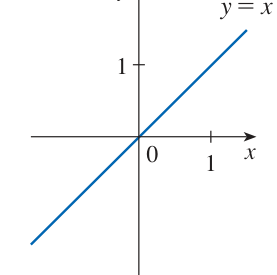
\includegraphics[width=0.185\linewidth]{images/p0062_fig4.png}\hfill
        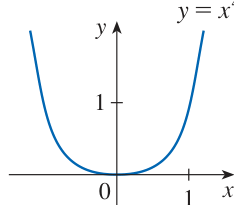
\includegraphics[width=0.185\linewidth]{images/p0062_fig5.png}
    \end{center}

    \vspace{-0.2cm}
    \noindent
    {\small \textbf{\textsf{HÌNH 11}}\quad Đồ thị của $f(x) = x^n$ với $n = 1, 2, 3, 4, 5$}

    \vspace{0.29cm}
    \noindent
    Dạng tổng quát của đồ thị hàm số $f(x) = x^n$ phụ thuộc vào việc $n$ là số chẵn hay số lẻ. Nếu $n$ là số chẵn, thì $f(x) = x^n$ là một hàm số chẵn và đồ thị của nó tương tự parabol $y = x^2$. Nếu $n$ là số lẻ, thì $f(x) = x^n$ là một hàm số lẻ và đồ thị của nó tương tự đồ thị của $y = x^3$. Tuy nhiên, hãy lưu ý từ Hình 12 rằng khi $n$ tăng lên, đồ thị của $y = x^n$ trở nên phẳng hơn ở lân cận $0$ và dốc hơn khi $|x| \geqslant 1$. (Nếu $x$ nhỏ, thì $x^2$ sẽ nhỏ hơn, $x^3$ thậm chí còn nhỏ hơn nữa, $x^4$ lại càng nhỏ hơn, v.v.)

    \vspace{0.16cm}
    \noindent
    \begin{center}
        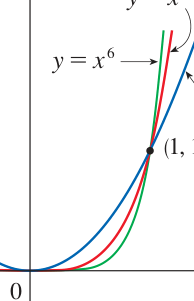
\includegraphics[width=0.48\linewidth]{images/p0062_fig6.png}\hfill
        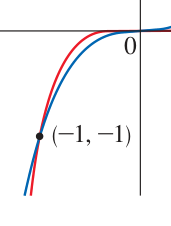
\includegraphics[width=0.48\linewidth]{images/p0062_fig7.png}
    \end{center}

    \vspace{0.16cm}
    \noindent
    \textbf{\textsf{(ii)}} $\boldsymbol{a = 1/n}$, \textbf{trong đó} $\boldsymbol{n}$ \textbf{là một số nguyên dương}

    \vspace{0.12cm}
    \noindent
    Hàm số $f(x) = x^{1/n} = \sqrt[n]{x}$ được gọi là một \textbf{hàm căn thức} (\textit{root function}). Với $n = 2$, đây là hàm căn bậc hai $f(x) = \sqrt{x}$, có tập xác định là $[0, \infty)$ và có đồ thị là nửa trên của parabol
\end{minipage}